\section{Method: placing a scene from its concept}\label{method-placing-a-scene-from-its-concept}

\subsection{The concept and its objects}\label{the-concept-and-its-objects}

A place begins, as before, with a concept picture the creator has locked. It is no longer read into rows, counts and a plan. SAM 3, run on a local graphics card, segments the whole picture into objects, each with its pixel box, mask and the word that found it, and an instance that duplicates a surer one under another word is dropped. These objects are the placing agent's list of what the scene must contain; how many there are and where they stand is the agent's to read from the picture, checked against the render.

\subsection{Kit placement and the concept-view compare loop}\label{kit-placement-and-the-concept-view-compare-loop}

The scene is built by a coding agent, Claude Code \citep{claudecode}, through one command-line tool, \texttt{place\_build}, whose steps lay and adjust a plain OpenUSD stage in metres. Every object it lays is a score\_lib entry copied whole into the place: modular kit pieces, models, the dome shells and tunnels, a switchback stair core of real size (0.167 m risers and 0.28 m treads), chamfered building blocks with window openings, lamps and sky domes. A surface step binds a library material over an object or one of its parts, so a model's baked colour never shows where the library has a better finish. Many steps run in one process on one open stage, so a complete relayout takes seconds.

The agent then renders the concept's own view, a camera it sets to match the concept's composition, through Blender's Cycles renderer \citep{blender}, and reads the render beside the concept. A review step renders a contact sheet of the same scene in one call: a plan section 2.4 m above the floor with a metre grid and object names, four corner views, eye-height views from each door, close-ups of each compartment, the concept in a corner and any physics fault boxed in red. From these the agent decides the next correction, such as moving a cluster of props to the side of the room where the concept shows them, changing a dome's height, or swapping a model that reads wrongly. Nothing in the tool judges the scene; it only lays, measures and renders, and the loop ends when the render reads as the concept, with the same room, layout, main objects and mood, while details may differ.

\subsection{One library, one palette a place}\label{one-library-one-palette-a-place}

Everything a place shows comes from score\_lib, and the usable content of the earlier method, the models that had passed their checks, its procedural materials and its code-made kits, was moved there before the old stages were removed. Because scans and models from many sources look inconsistent side by side, each place takes in one scene surface library, a set of procedural material variants written as ProcFunc recipes \citep{raistrick2026procfunc} on Infinigen's shaders \citep{raistrick2023infinigen} in the place's palette tokens, with their wear and dirt. Shells, floors and repainted parts take their finishes from it, so that they share the look of the props.

\subsection{Props made with TRELLIS.2}\label{props-made-with-trellis.2}

A prop that the library lacks, or whose model reads worse than the picture, is made with TRELLIS.2 \citep{trellis2}, an open image-to-3D model released under the MIT licence, from a crop of the concept cut out by its SAM 3 mask or from the close-up of an earlier model. The model is generated on the creator's own 16 GB graphics card, built from source with its dependencies at pinned commits, in about three minutes per prop under load. The new mesh is fitted over the model it replaces by quarter turns and one uniform scale, minimising the two-way distance between their point sets. Its own paint is then graded 60 percent of the way toward the nearest palette token, and a colour group that stays far from every token is reported so that the agent can repaint it from the library. Finally the model is made simulation-ready. CoACD \citep{wei2022coacd} decomposes it into convex hulls for collision, its mass is the hulls' outer surface times the material class's sheet thickness and density, and friction and restitution follow the class. On six camp props the masses lie beside those of the earlier models (a crate of 4.0 against 2.6 kg, a desk of 44 against 42 kg, a chair of 5.1 against 4.7 kg), but steel frames come out heavy, because a hull closes over a frame's gaps. Figure 2 compares the two routes on the same pictures.

\begin{figure}
\centering
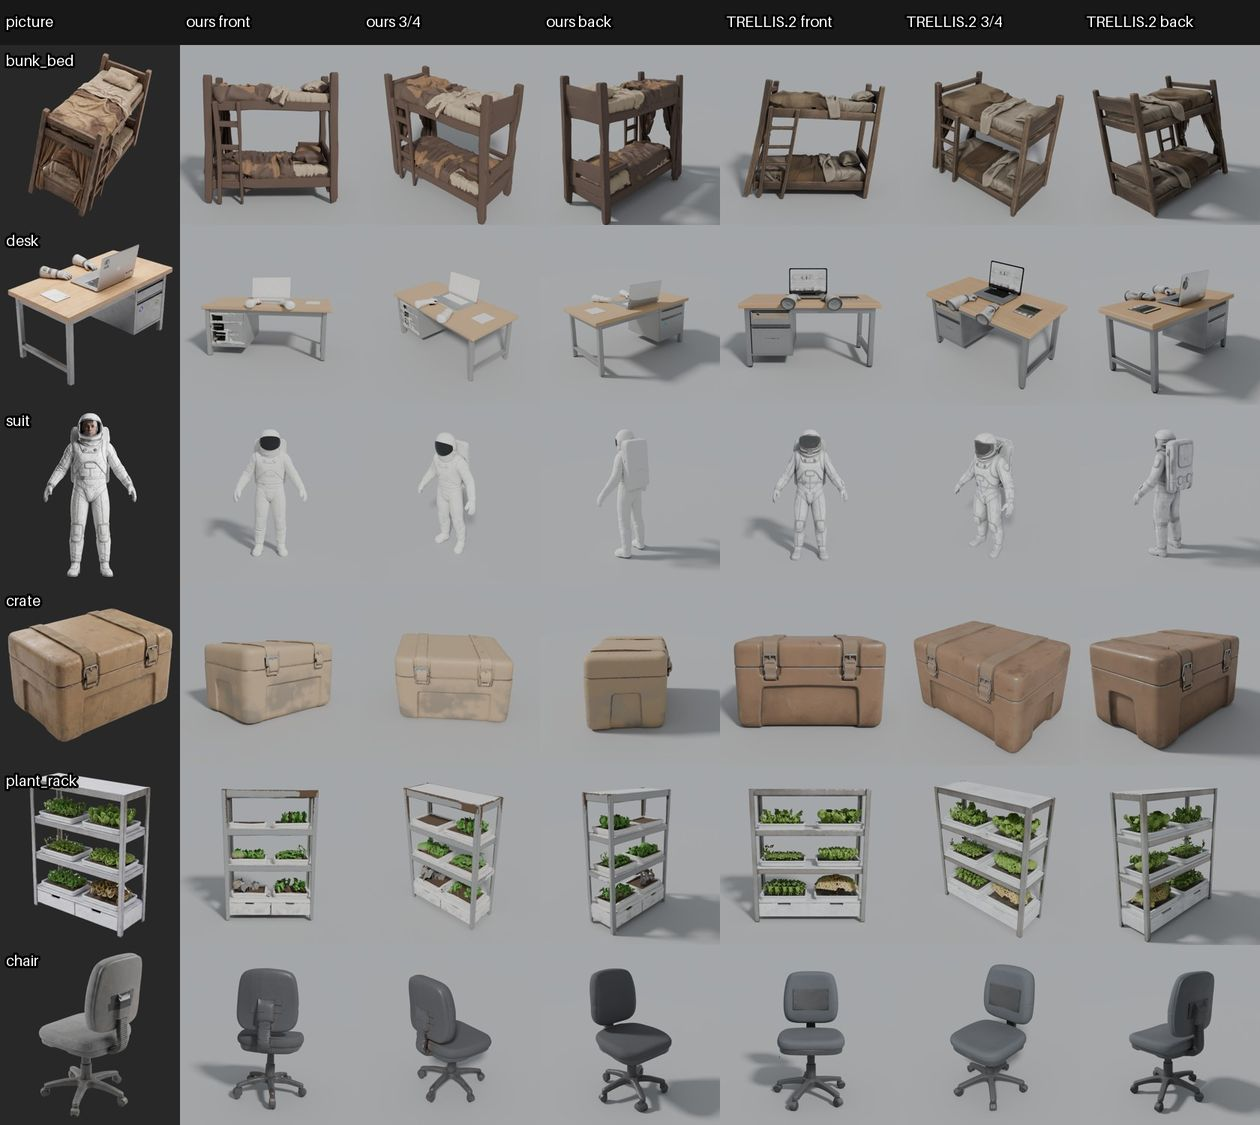
\includegraphics[width=0.88\linewidth,height=\textheight,keepaspectratio,alt={The same six camp pictures (left) made by SCORE's earlier picture-made route (centre three columns) and by TRELLIS.2 (right three columns), each from the front, three-quarter and back. The building agent judged the TRELLIS.2 model the better match on five of the six.}]{figures/trellis2.jpg}
\caption{The same six camp pictures (left) made by SCORE's earlier picture-made route (centre three columns) and by TRELLIS.2 (right three columns), each from the front, three-quarter and back. The building agent judged the TRELLIS.2 model the better match on five of the six.}
\end{figure}

\subsection{Real terrain}\label{real-terrain}

Outdoor places stand on real ground. A terrain entry is a heightfield read from a public-domain digital terrain model of the HiRISE camera on the Mars Reconnaissance Orbiter \citep{mcewen2007hirise} (NASA/JPL/University of Arizona), fetched by range requests rather than as a whole file, dense near the place and sparser toward a horizon that bends with the planet. A building's site is levelled to its laid height and eased into the surrounding relief, and loose rocks are set onto the relief at their own footprints.

\subsection{The physics-readiness check}\label{the-physics-readiness-check}

A scene that reads as its concept may still be one a simulator cannot use, and every round of the compare loop therefore ends with a physics-readiness check. It assigns each object a role from the scene (ground, shell, structure, connector, door, prop, mount, person or far scenery) and reports every fault by object and kind. Each object must rest on a support within 3 cm and stand in balance, and sampled points of its surface must not lie inside another object. A door must lie in an opening, with its outline within 5 cm of the opening's edge, and a connector such as a tunnel must meet the structures it joins within 30 cm with a floor along its length. Every person's feet must touch a floor within 1 cm, and no body may be torn. The walkers' floor is computed as Recast-style walkable spans \citep{recast} with every solid's footprint removed and eroded to a way at least 0.9 m wide, and it must link every spot a walker is sent to. Ground and fixed pieces more than 20 m beyond anything a walker can reach count as scenery and are left out of every measure. Finally, the props are released as free bodies in MuJoCo 3.15 for one simulated second at Earth gravity, one small model per object with its static neighbours, and any prop that falls, tips or drifts is a fault. Every fault kind has a planted counterpart in the check's test, which must be reported by name. The check never moves anything; the agent corrects and runs it again.

\subsection{A builder tournament}\label{a-builder-tournament}

A single agent's layout depends on its early choices, so each place was built by three independent builders that used the same tools, library and check, each trying its own layout. Judging agents compared their concept-view renders with the concept, the best one was kept, and a final builder refined it with the strongest elements of the others. The tournament's per-builder scores were not kept as a record; only the winning scenes and their checks were.
